\documentclass[final,inline,a4paper,narroweqnarray]{ieee}
% In order to use the figure-defining commands in ieeefig.sty...
\usepackage{ieeefig}
% To use utf8 encoding
\usepackage[T1]{fontenc}
\usepackage[utf8]{inputenc}
\usepackage[spanish]{babel}
% to place figures
\usepackage{float}
\usepackage{graphicx}
% dont use geometry package
%\usepackage{geometry}
\begin{document}

%----------------------------------------------------------------------
% Title Information, Abstract and Keywords
%----------------------------------------------------------------------
\title[TP N$^o$ 1: Wiretapping]{%
Trabajo Práctico N$^o$ 1: Wiretapping}

% format author this way for journal articles.
\author[Barrios, Benegas, Caravario, Rodriguez]{%
	Leandro Ezequiel Barrios,
	\and
	Gonzalo Benegas,
	\and
	Martin Caravario,
	\and
	Pedro Rodriguez
}

% make the title
\maketitle

% do the abstract
\begin{abstract}

En el presente Trabajo Práctico utilizaremos algunas de las técnicas
provistas por la teoría de la información para estudiar y analizar
algunas redes de información. El objetivo será distinguir diversos
aspectos de la red de manera analítica. Para cumplir con nuestro
objetivo, haremos uso de dos herramientas modernas de manipulación y
análisis de paquetes: Wireshark y Scapy.

\end{abstract}

% start the main text ...

%----------------------------------------------------------------------
% SECTION I: Introduction
%----------------------------------------------------------------------
\section{ Introducción }

Construimos una herramienta que hace uso de la función
\texttt{``sniff''}, provista por la librería \textbf{Scapy} de
Python. Esta nos permitió activar el \texttt{modo promiscuo}, o
\texttt{monitor} en el caso de las placas wireless. Esto nos permitió
escuchar la red durante cierto tiempo, obteniendo todos los paquetes
que llegaban a nuestra placa de red. A partir de estos datos que
guardamos en un archivo \texttt{pcap}, se definieron dos fuentes de
información, con las cuales fuimos capaces de encontrar nodos y
protocolos distinguidos en la red. Para su visualización, elegimos la
realización de gráficos de torta e histogramas, ya que los
consideramos los más apropiados.

Para cada una de las mediciones consideramos las siguientes fuentes:
\begin{itemize}

  \item $S = \{s_{1} \dots s_{n}\}$, provista por la cátedra, donde
  $s_{i}$ es el valor del campo \emph{type} de cada paquete de capa
  2.

  \item $S_{1} = \{s_{1} \dots s_{n}\} $, determinada por nosotros,
  donde $s_i$ es el valor del campo destino (\texttt{IP}) cada paquete
  de capa 2 de tipo \texttt{ARP}.

\end{itemize}

\medskip

Para entender qué es lo que se obtendrá al efectuar estas mediciones,
hay que aclarar que \texttt{ARP} es un protocolo de la capa de enlace
de datos, responsable de encontrar la dirección de capa 2
(\texttt{Ethernet MAC}) que corresponde a una determinada dirección IP
(dirección de capa 3 de red).

Es decir, cada vez que un host quiere comunicarse con otro y su
dirección \texttt{MAC} no se encuentra dentro de su tabla
\texttt{ARP}, debe enviar un paquete who-has broadcast para determinar
la dirección \texttt{MAC} del host destino. De este modo, todos los
hosts del dominio de colisión de la máquina en la que se efectúa la
medición reciben dicho paquete, siendo respondido el mismo únicamente
por el host requerido, mediante un paquete \emph{reply}.

Para distinguir \emph{nodos} (símbolos) en este contexto, tomamos a
aquellos cuya probabilidad de aparición era alta, de forma tal que la
información provista por el mismo fuera menor a la entropía de la
fuente a la cuál el símbolo pertenecía.

Tomamos esta decisión porque, según Shannon, el nivel de entropía de una
fuente habla de la máxima compresibilidad de cada bit en un mensaje enviado
con una codificación óptima ($H(F) \leq L(C)$). Luego, si la
fuente presenta símbolos cuya cantidad de información está
por debajo de la entropía, son símbolos que tienen mucha probabilidad de
aparecer en un mensaje en comparación con los otros, y podría ser
conveniente representar a estos símbolos con menos bits que al resto, para
así disminuir la longitud media del código. Por ejemplo, supongamos que
enviamos números binarios, y sabemos que el símbolo $X = "00000000"$ aparece en
los mensajes la mitad del tiempo y que el resto de las tiras pueden aparecer
todas con la misma
probabilidad. Entonces, $X$ brindaría una cantidad de información por debajo
de la entropía, y convendría representar a esa tira simplemente con un $0$,
y al resto de las tiras prefijarlas con el $1$. De esta manera, se ahorraría
en promedio $7$.$1/2+(-1)$.$1/2 = 3$ bits en cada mensaje.

Entonces, también analizaremos las entropías de las fuentes en cada una
de las escuchas de red realizadas, y trataremos
de concluir cuál de las dos fuentes elegidas es \emph{más compresible}.

\subsection{Casa}

  Esta siguiente medición fue realizada en una red LAN hogareña, en el
  horario de las 15:00 hs, por un lapso de 3 hs. La herramienta
  utilizada fue la indicada en el enunciado del trabajo. A esta LAN
  hubo conectadas 5 computadoras, una impresora y 3 celulares al
  momento de la medición.

\subsection{Techint}

  Esta medición fue realizada en la empresa Techint, en el horario de
  las 11:00 am, por un lapso de 30 minutos. Se utilizó la herramienta
  desarrollada en el ejercicio anterior. Se desconoce la cantidad de
  computadoras o la topología de la red medida. La conexión a la red
  fue efectuada mediante un cable de ethernet.


\subsection{Hyundai}

  Esta medición fue realizada en la empresa Hyundai Motor Argentina,
  en horario laboral, durante 5 horas. El edificio en donde se realizó
  la medición, cuenta con unos 30 estaciones de trabajo fijas (PC
  Desktop), y 10 Notebooks, distribuídas a través de los pisos del
  edificio. La red tiene, además, un \textbf{switch de nivel 2} por
  sector, al que se encuentran conectados los dispositivos que
  pertenecen al departamento. A su vez, cada uno de estos está
  conectado a un \textbf{switch de nivel 3} a través de un
  \textbf{enlace Gigabit punto a punto}. A su vez, hay al menos un
  \textbf{access point} en cada uno de los sectores de la empresa, al
  cual se conectan la mayoría de los dispositivos móviles de los
  empleados. También hay diversos dispositivos, impresoras de red,
  lectores de códigos de barras inalámbricos, cámaras IPs, teléfonos
  IPS, entre otros, conectados a los
  \textbf{switches} o \textbf{access point} de cada sector.

  A su vez, existen varios servidores conectados mediante un enlace
  \textbf{PPP} al switch principal, que proveen de diversos servicios a las
  estaciones de trabajo, por ejemplo: active directory, samba, correo
  electrónico, backup, acceso a bases de datos, acceso a sistemas,
  telefonía IP, acceso a internet, etc.

  La conexión fue realizada mediante una conexión cableada
  \textbf{PPP} entre el switch principal, y la computadora corriendo
  el sniffer, lo que nos permite suponer que pese a activar el modo
  promiscuo, sólo llegarán hasta la placa de red aquellos paquetes que
  se encuentren dentro de su dominio de broadcast.

\subsection{Laboratorios DC}



%----------------------------------------------------------------------
% SECTION II: Desarrollo - Fuente S
%----------------------------------------------------------------------
\section{Desarrollo - Fuente S}
  %--------------------------------------------------------------------
  % SUBSECTION II-A: CASA
  %--------------------------------------------------------------------
  \subsection{Casa}

   Los resultados obtenidos fueron los siguientes

\begin{table}[h]\begin{center}
    \begin{tabular}{|c|c|c|}
    \hline
    \textbf{Protocolo} & \textbf{Informacion} & \textbf{Frecuencia} \\ \hline
    \texttt{802.1X    }& 15.38       & 0.00\%     \\ \hline
    \texttt{IPv6      }& 9.59        & 0.13\%     \\ \hline
    \texttt{ARP       }& 6.65        & 0.99\%     \\ \hline
    \texttt{IPv4      }& 0.02        & 98.87\%    \\ \hline
    \end{tabular}
    \caption{S: Casa - Mediciones}
    \label{casa-s-table}
\end{center}\end{table}

    El protocolo que más fue escuchado fue \texttt{IPv4}, tal como se
    observa en la figura \ref{marto-casa-3hs-s-pie}, la cantidad de
    paquetes  de este tipo fue del 98\% mientras que la de paquetes
    \texttt{ARP} fue del 1\%. Esto permite concluir que en el caso de
    la red hogareña, el overhead del tipo \texttt{ARP} en un tiempo de
    3 horas es practicamente nulo, con respecto al total de paquetes
    de la red.

    %------------------------------------------------------------------
    % TORTA CASA
    %------------------------------------------------------------------

    \begin{figure}[ht]\begin{center}
      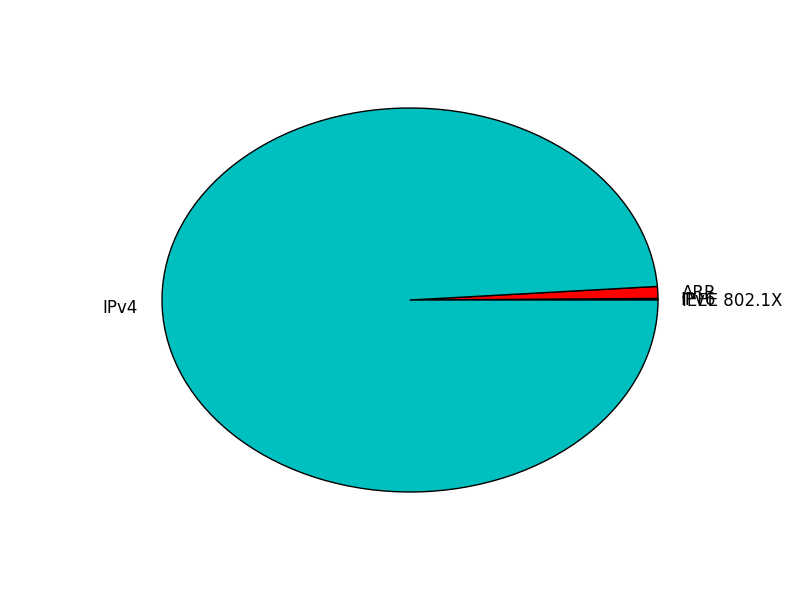
\includegraphics[width=0.5\textwidth]{%
      ../output/marto-casa-3hs-s-pie.png}
      \vspace{-3em}
      \caption{S: Casa - Torta}
      \label{marto-casa-3hs-s-pie}
    \end{center}\end{figure}

    La entropía de la fuente propuesta es de 0.095, lo que indica que
    los símbolos emitidos por la fuente son muy previsibles. Esto se
    puede observar en la figura \ref{marto-casa-3hs-s-histogram},
    donde deja por debajo de ella al protocolo \texttt{IPv4} que, al
    presentar una mayor probabilidad de aparición en la fuente,
    provoca que la información que aporte sea poca y lo destaque como
    nodo distinguido. A diferencia de \texttt{IPv4}, podemos encontrar
    al protocolo \texttt{802.1X} que al tener poca probabilidad de
    aparición $(2.35 * 10^-5)$, aporta mucha información, siendo el
    protocolo que más aporta.

    %------------------------------------------------------------------
    % HISTOGRAMA CASA
    %------------------------------------------------------------------

    \begin{figure}[ht]\begin{center}
     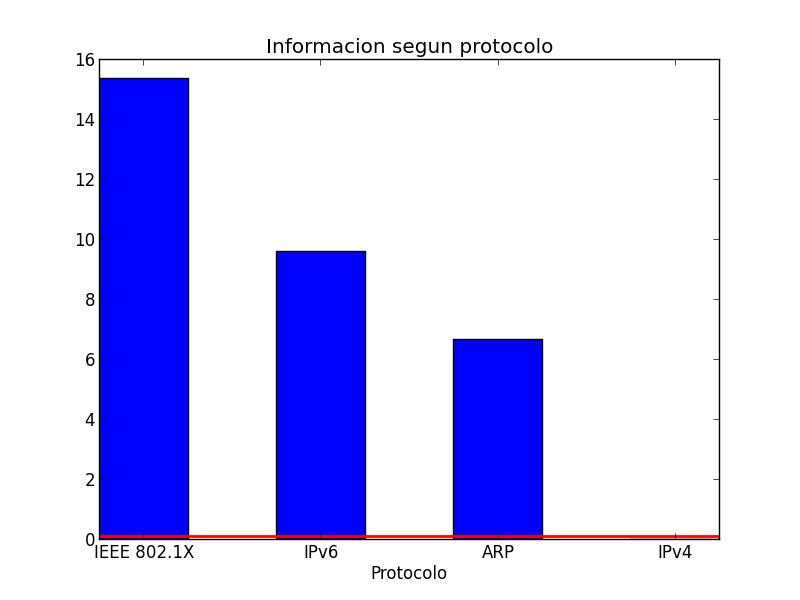
\includegraphics[width=0.5\textwidth]{%
      ../output/marto-casa-3hs-s-histogram.png}
      \caption{S: Casa - Histograma}
      \label{marto-casa-3hs-s-histogram}
    \end{center}\end{figure}

    %------------------------------------------------------------------
    % SUBSECTION II-B: TECHINT
    %------------------------------------------------------------------
    \subsection{Techint}

    Los resultados se pueden ver en la
    \textbf{tabla\ref{techint-s-table}}.

    \begin{table}\begin{center}
      \begin{tabular}{|c|c|c|}
      \hline
      \textbf{Protocolo} & \textbf{Informacion} & \textbf{Frecuencia} \\ \hline
      \texttt{ARP       }& 3.03        & 12.26\%    \\ \hline
      \texttt{IPX       }& 6.40        & 1.19\%     \\ \hline
      \texttt{IPv4      }& 0.82        & 56.55\%    \\ \hline
      \texttt{802.3     }& 2.74        & 14.92\%    \\ \hline
      \texttt{IPv6      }& 2.74        & 14.93\%    \\ \hline
      \texttt{LLDP      }& 9.30        & 0.16\%     \\ \hline
      \end{tabular}
      \caption{S: Techint - Mediciones}
      \label{techint-s-table}
    \end{center}\end{table}

    El protocolo que más aparece en este escenario es \texttt{IPv4},
    tal como se observa en la figura \ref{techint-s-pie}, haciendo que
    su probabilidad sea la mayor. Esto se ve reflejado en la figura
    \ref{techint-s-histogram}, en la cual se puede ver como afecta la
    frecuencia de aparición del protocolo a la información que este
    provee.

    %------------------------------------------------------------------
    % TORTA TECHINT
    %------------------------------------------------------------------

    \begin{figure}[ht]\begin{center}
      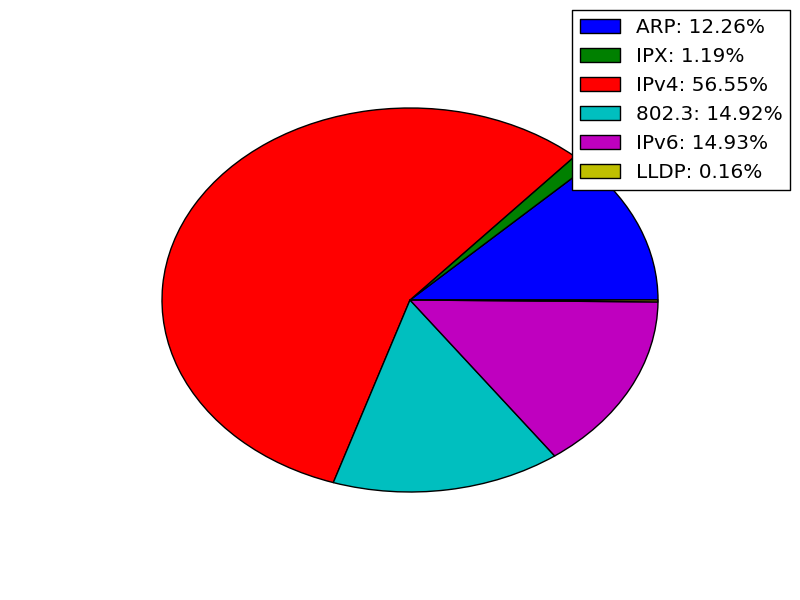
\includegraphics[width=0.5\textwidth]{%
      ../output/techint-s-pie.png}
      \vspace{-3em}
      \caption{S: Techint - Torta}
      \label{techint-s-pie}
    \end{center}\end{figure}

    En este caso el nodo distinguido es el protocolo \texttt{IPv4},
    pues la información que provee es menor a la entropía de la fuente
    utilizada(1.74) , y además es el único que está por debajo de
    ella. El protocolo que más información aporta es \texttt{LLDP}, ya
    que su frecuencia de aparición(0.15\%) es la menor en la medición
    tomada. Esto genera que las pocas veces que aparece aporte más
    información en comparación con los protocolos que más aparecen,
    como por ejemplo \texttt{IPv4} cuyo porcentaje de aparición sobre
    el total es del 56\% tal como se observa en la figura
    \ref{techint-s-pie}.

    %------------------------------------------------------------------
    % HISTOGRAMA TECHINT
    %------------------------------------------------------------------

    \begin{figure}[ht]\begin{center}
      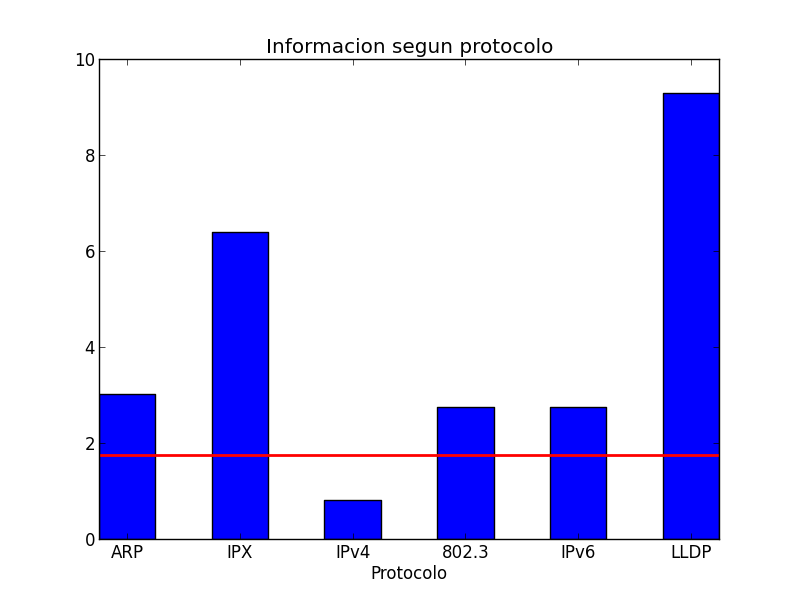
\includegraphics[width=0.5\textwidth]{%
      ../output/techint-s-histogram.png}
      \caption{S: Techint - Histograma}
      \label{techint-s-histogram}
    \end{center}\end{figure}

    También se puede observar en la figura \ref{techint-s-pie}, la
    gran cantidad de paquetes de tipo \texttt{ARP} (12\%) que
    aparecen, en comparación con los de tipo \texttt{IPv6} (15\%) y
    \texttt{802.3} (14\%), que se encuentran en segundo lugar y tercer
    lugar respectivamente. Esto demuestra el overhead del protocolo
    \texttt{ARP} sobre el total de paquetes escuchados.

    El protocolo que mas aparece en este escenario es \texttt{IPv4}, tal
    como se observa en la figura \ref{techint-s-pie}, haciendo que
    su probabilidad sea la
    mayor. Esto se ve reflejado en la figura \ref{techint-s-histogram},
    en la cual se puede ver como
    afecta la frecuencia de aparición del protocolo a la información
    que este provee.


    En este caso el nodo distinguido es el protocolo \texttt{IPv4},
    pues la información que provee es menor a la entropía de la fuente
    utilizada(1.74) , y además es el único que está por debajo de ella. El
    protocolo que mas información aporta es \texttt{LLDP}, ya que
    su frecuencia de aparición(0.15\%) es la menor en la medición tomada. Esto
    genera que las pocas veces que aparece aporte mas información en
    comparación con los protocolos que más aparecen, como por ejemplo
    \texttt{IPv4} cuyo porcentaje de aparición sobre el total es del 56\%
    tal como se observa en la figura \ref{techint-s-pie}.

  %--------------------------------------------------------------------
  % SUBSECTION II-C: HYUNDAI
  %--------------------------------------------------------------------
  \subsection{Hyundai}

    \begin{table}\begin{center}
      \begin{tabular}{|c|c|c|}
      \hline
      \textbf{Protocolo}   & \textbf{Frecuencia} & \textbf{Informacion}\\ \hline
      \texttt{ARP         }& 0.75\%     & 7.06       \\ \hline
      \texttt{IPX         }& 0.01\%     & 13.41      \\ \hline
      \texttt{IPv4        }& 98.82\%    & 0.02       \\ \hline
      \texttt{IEEE\_26734 }& 0.00\%     & 16.21      \\ \hline
      \texttt{802.3       }& 0.15\%     & 9.38       \\ \hline
      \texttt{IPv6        }& 0.27\%     & 8.55       \\ \hline
      \texttt{LLDP        }& 0.01\%     & 13.71      \\ \hline
      \end{tabular}
      \caption{S: Hyundai - Mediciones}
      \label{hyundai-s-table}
    \end{center}\end{table}

    Se pueden apreciar los resultados de las mediciones en la tabla
    \ref{hyundai-s-table}. Lo primero que se observa es una muy fuerte
    predominancia de paquetes de protocolo IPv4.

    A priori, según los resultados de esta medición, parecería que
    \texttt{ARP} no impone un overhead considerable. Tomando este
    hecho, decidimos comparar esta medición con el resto, y buscar en
    qué cosas se diferencian, con el fin de encontrar a qué se debe
    esta situación de alta eficiencia. Encontramos dos grandes
    diferencias con el resto de las mediciones:

    \begin{itemize}

    \item El largo tiempo de medición / la alta cantidad de paquetes
    capturados.

    \item La medición, realizada mediante placa ethernet en modo
    promiscuo, no tiene el alcance de una medición wireless en modo
    monitor.

    \item La red switcheada, que encapsula los dominios de broadcast y
    colisión, reduciendo sensiblemente el tráfico de la red.

    \end{itemize}

    De estos tres puntos, el tiempo de medición como amortiguador del
    overhead de ARP resulta sumamente interesante, en parte debido a
    que las limitaciones de la medición en modo promiscuo eran sabidas
    de antemano, y son inevitables, y el beneficio de una red de
    switches en cascada fue explicado en clase. Además, es una
    conjetura fácil de poner a prueba. Basta particionar los datos de
    una misma captura, en intervalos de tiempo cada vez mayores, para
    comprobar si efectivamente al aumentar el tiempo de medición, se
    produce el efecto esperado.

    Tomando la medición original, se la cortó en intervalos de 1
    minuto, 5 minutos, 10 minutos, 20 minutos y 30 minutos. En las
    figuras \ref{hyundai-1-s-pie}, \ref{hyundai-5-s-pie},
    \ref{hyundai-10-s-pie}, \ref{hyundai-20-s-pie} y
    \ref{hyundai-30-s-pie} se puede ver claramente una progresión, en
    la que a medida que el tiempo de medición aumenta, el overhead de
    ARP disminuye.

    %------------------------------------------------------------------
  	% GRAFICOS HYUNDAI - TIEMPO
    %------------------------------------------------------------------
    \begin{figure}[h]\begin{center}
      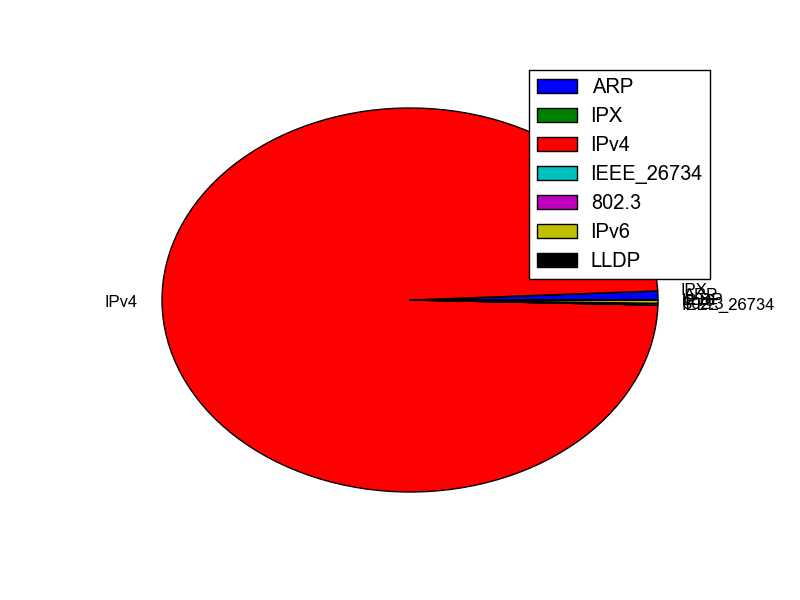
\includegraphics[width=0.5\textwidth]{%
      ../output/hyundai-s-pie.png}
      \vspace{-3em}
      \caption{S: Hyundai - Torta}
      \label{hyundai-s-pie}
    \end{center}\end{figure}

    %------------------------------------------------------------------
    % HISTOGRAMA HYUNDAI
    %------------------------------------------------------------------
    \begin{figure}[H]\begin{center}
      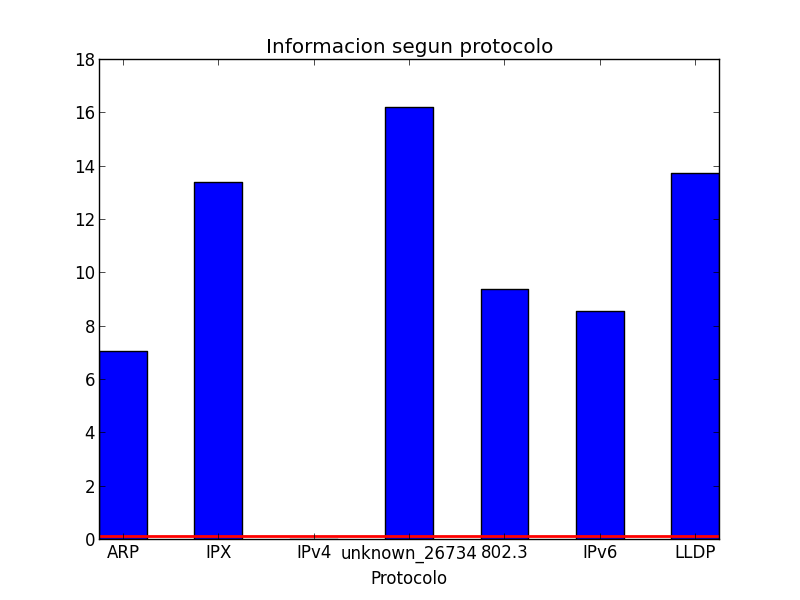
\includegraphics[width=0.5\textwidth]{%
      ../output/hyundai-s-histogram.png}
      \caption{S: Hyundai - Histograma}
      \label{hyundai-s-histogram}
    \end{center}\end{figure}

    Se realizó además un gráfico de histograma (\emph{fig.
    \ref{hyundai-s-histogram}}) y un gráfico de torta (\emph{fig.
    \ref{hyundai-s-pie}}), que permiten apreciar la relación entre los
    distintos protocolos de una forma visual e inmediata.

    %------------------------------------------------------------------
    % HYUNDAI TIEMPO - PROGRESION
    %------------------------------------------------------------------
    \begin{figure}[H]\begin{center}
      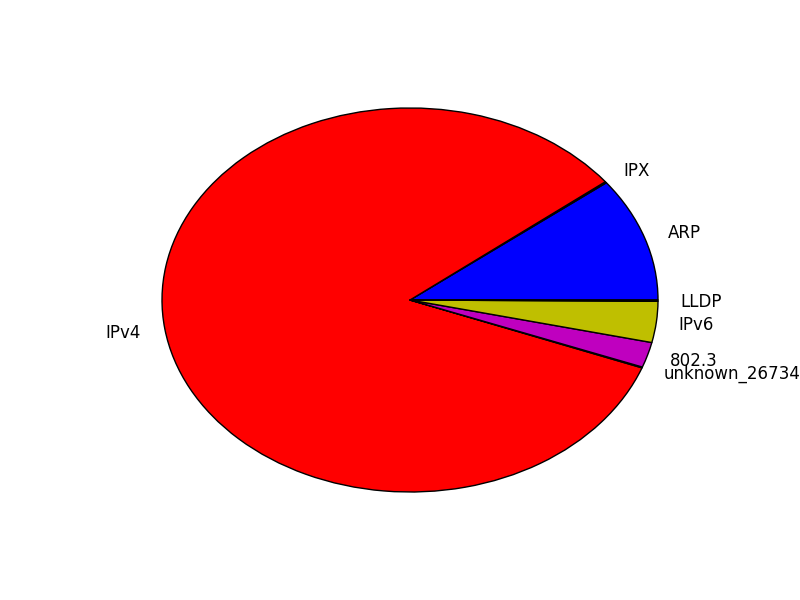
\includegraphics[width=0.5\textwidth]{%
      ../output/hyundai-1-s-pie.png}
      \vspace{-3em}
      \caption{S: Hyundai - Torta (1 minuto)}
      \label{hyundai-1-s-pie}
    \end{center}\end{figure}
    %
    \begin{figure}[H]\begin{center}
      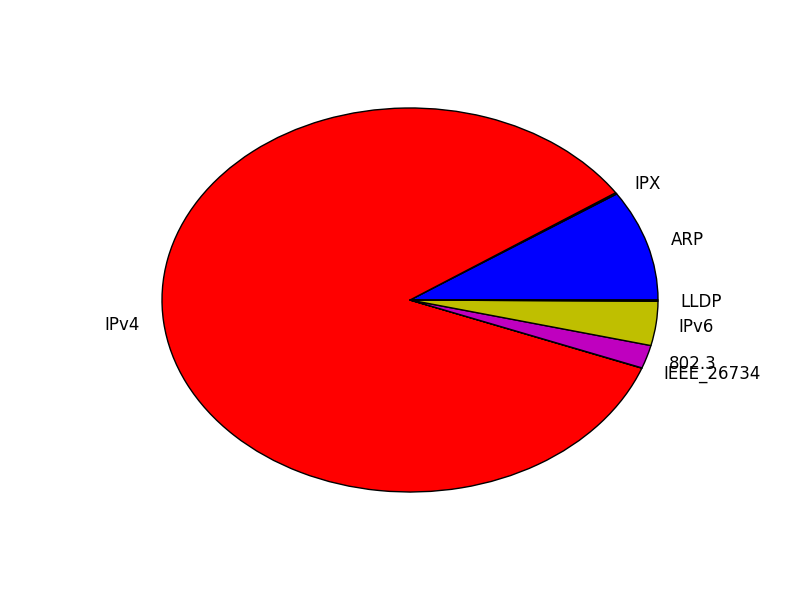
\includegraphics[width=0.5\textwidth]{%
      ../output/hyundai-5-s-pie.png}
      \vspace{-3em}
      \caption{S: Hyundai - Torta (5 minutos)}
      \label{hyundai-5-s-pie}
    \end{center}\end{figure}
    %
    \begin{figure}[H]\begin{center}
      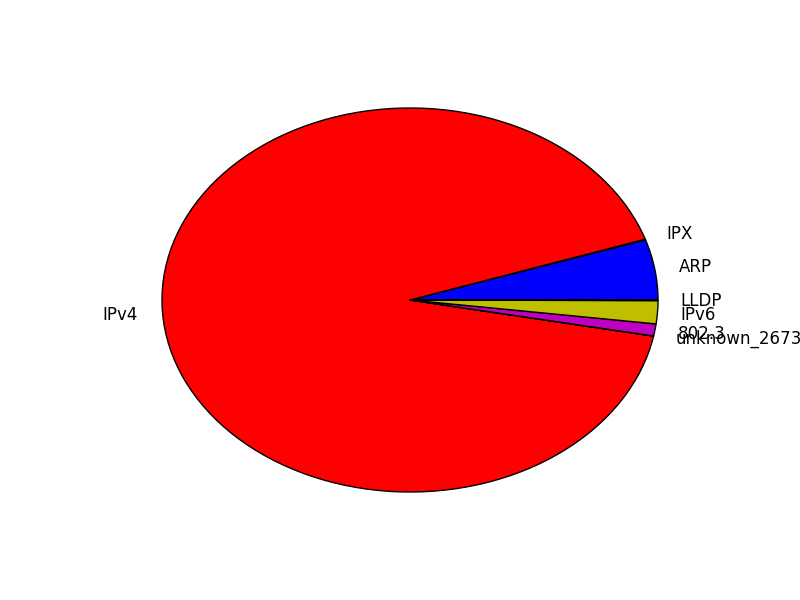
\includegraphics[width=0.5\textwidth]{%
      ../output/hyundai-10-s-pie.png}
      \vspace{-3em}
      \caption{S: Hyundai - Torta (10 minutos)}
      \label{hyundai-10-s-pie}
    \end{center}\end{figure}
    %
    \begin{figure}[H]\begin{center}
      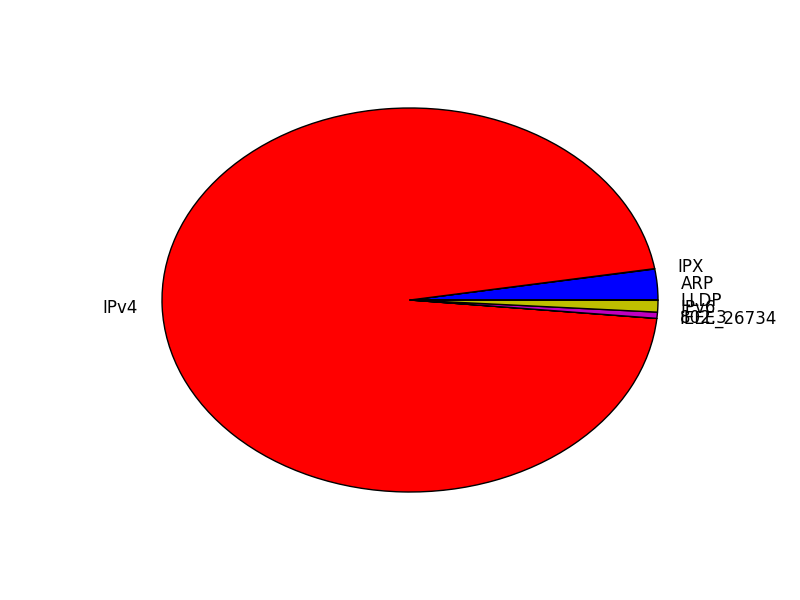
\includegraphics[width=0.5\textwidth]{%
      ../output/hyundai-20-s-pie.png}
      \vspace{-3em}
      \caption{S: Hyundai - Torta (20 minutos)}
      \label{hyundai-20-s-pie}
    \end{center}\end{figure}
    %
    \begin{figure}[H]\begin{center}
      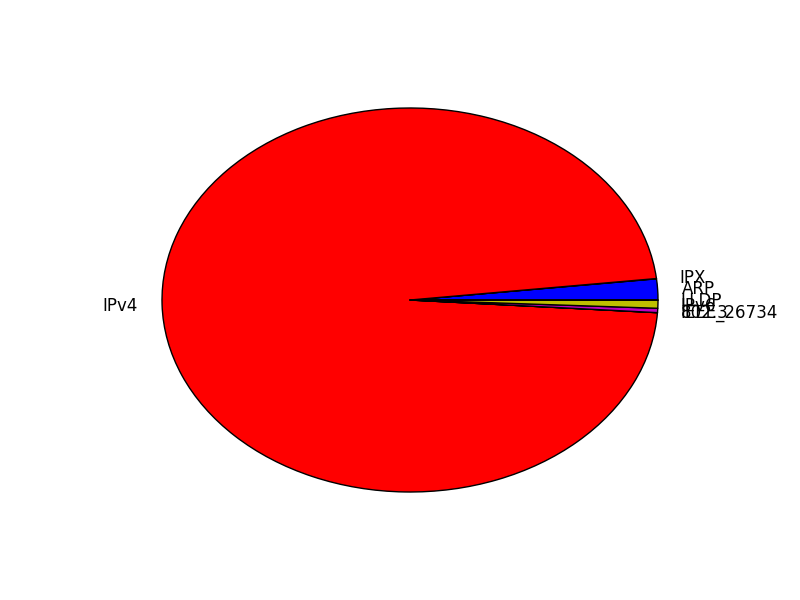
\includegraphics[width=0.5\textwidth]{%
      ../output/hyundai-30-s-pie.png}
      \vspace{-3em}
      \caption{S: Hyundai - Torta (30 minutos)}
      \label{hyundai-30-s-pie}
    \end{center}\end{figure}
    %

  %
  %--------------------------------------------------------------------
  % SUBSECTION II-D: LABORATORIOS DC
  %--------------------------------------------------------------------
  %
  \subsection{Laboratorios DC}

    Esta medición fue realizada en los laboratorios del departamento de
    computación, en el horario de las 17 hs, por un lapso de 30 minutos.
    Se utilizó la herramienta explicada previamente. La red cuenta con 175
    computadoras, y se desconoce la cantidad de celulares conectados a ella.
    Los resultados fueron los siguientes.

    \begin{table}\begin{center}
      \begin{tabular}{|c|c|c|}
      \hline
      \textbf{Protocolo} & \textbf{Informacion} & \textbf{Frecuencia} \\ \hline
      \texttt{IPv6      }& 4.25        & 5.26\%     \\ \hline
      \texttt{802.3     }& 6.41        & 1.17\%     \\ \hline
      \texttt{IPv4      }& 0.28        & 82.40\%    \\ \hline
      \texttt{ARP       }& 3.16        & 11.17\%    \\ \hline
      \end{tabular}
      \label{labos-dc-s-table}
      \caption{S: Laboratorios DC - Mediciones}
    \end{center}\end{table}

    %------------------------------------------------------------------
    % TORTA LABOS-DC
    %------------------------------------------------------------------
    \begin{figure}[ht]\begin{center}
      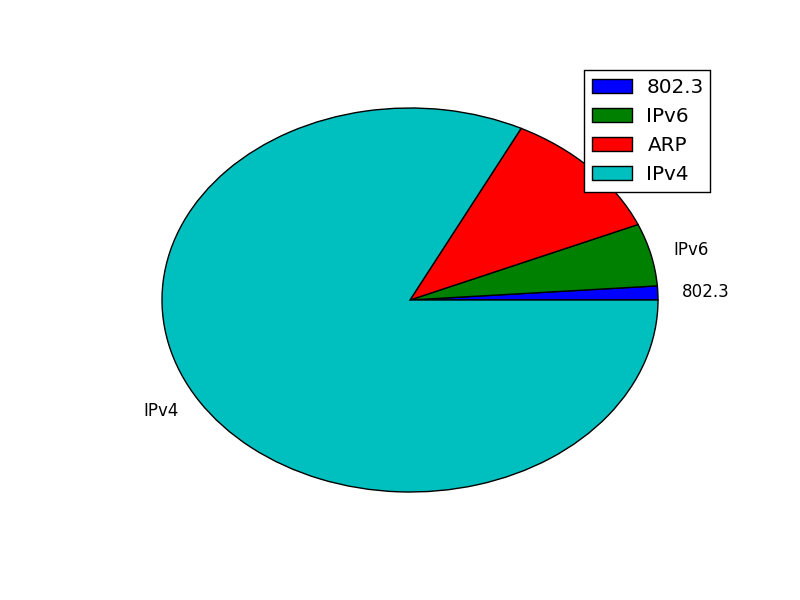
\includegraphics[width=0.5\textwidth]{%
      ../output/labos-dc-30m-s-pie.png}
      \vspace{-3em}
      \caption{S: Laboratorios DC - Torta}
      \label{labos-dc-30m-s-pie}
    \end{center}\end{figure}

    %------------------------------------------------------------------
    % HISTOGRAMA LABOS-DC
    %------------------------------------------------------------------
    \begin{figure}[ht]\begin{center}
      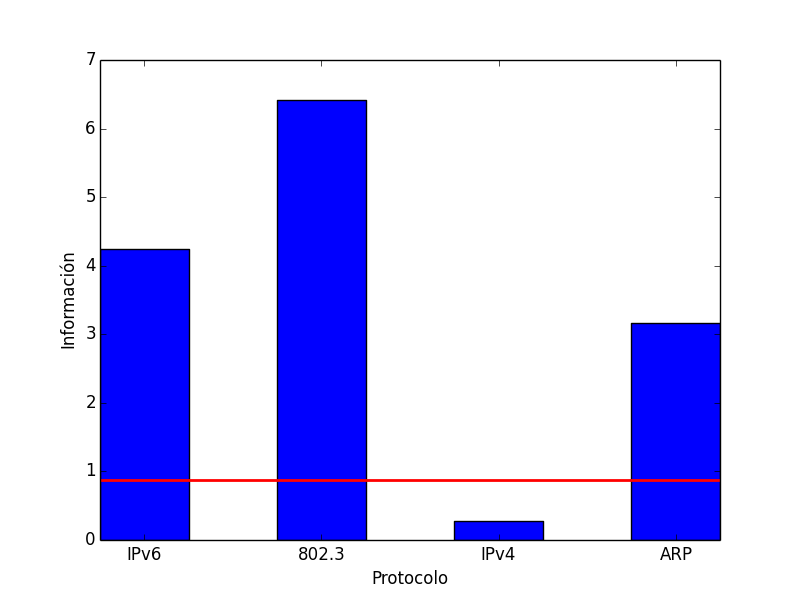
\includegraphics[width=0.5\textwidth]{%
      ../output/labos-dc-30m-s-histogram.png}
      \caption{S: Laboratorios DC - Histograma}
      \label{labos-dc-30m-s-histogram}
    \end{center}\end{figure}

    El protocolo que más se escuchó fue \texttt{IPv4}, tal como se
    observa en la figura \ref{labos-dc-30m-s-pie}, la cantidad de
    paquetes  de este tipo fue del 82\% mientras que la de paquetes
    \texttt{ARP} fue del 11\%. Se observa que el overhead del tipo
    \texttt{ARP} en un tiempo de 30 minutos es bajo pero no
    despreciable con respecto al total de paquetes de la red.

    La entropía de la fuente propuesta es de 0.882, como se observa en
    la figura \ref{labos-dc-30m-s-histogram}, dejando por debajo de
    ella al protocolo \texttt{IPv4} que, al presentar una mayor
    probabilidad de aparición en la fuente, provoca que la información
    que aporta sea poca y se destaque como nodo distinguido. Podemos
    encontrar al protocolo
    \texttt{802.3} que al tener poca probabilidad de aparición
    (1\%), aporta mucha información, siendo el protocolo que más
    información aporta.

    %------------------------------------------------------------------
    % SUBSECTION II-F: Conclusión
    %------------------------------------------------------------------
    \subsection{Conclusión}

    Notamos una fuerte tendencia del protocolo IPv4 frente al resto. Pese a que IPv6 ya se encuentra vigente hace años, es sabido el hecho de que su implementación aún no se ha extendido como se preveía. En algunas redes pudimos notar, sin embargo, una representación no negligible.

    Con respecto al overhead impuesto por el protocolo ARP, notamos que no es lo suficientemente significativo como para ser motivo de preocupación, sobretodo cuando la red tiene una alta participación de otros protocolos, en donde se puede notar que mientras ARP produce una carga que se podría considerar constante o periódica, debido a la tabla caché de ARP, las cargas impuestas por otros protocoles responden a la intensidad de uso de la red. ARP en cambio, no presenta esta particularidad.

    % HABLAR SOBRE EL PREDOMINIO DE IPV4 SOBRE IPV6 QUE TODAVIA NO ESTA BIEN IMPLEMENTADO EN
    % TODOS LADOS

    % IMPACTO DE ARP: SE PIERDE MUCHO TIEMPO EN PROTOCOLOS DE "MANTENIMIENTO" QUE NO APORTAN
    % INFORMACION

    % GRAN IMPACTO DE ARP EN LAPSOS CORTOS DE ESCUCHA, EN TIEMPOS LARGOS EL OVERHEAD BAJA
    %
    %
    % También se observa el gran predominio de \texttt{IPv4} sobre \texttt{IPv6},
    % el cual actualmente no esta implementado ni funcionando en todos
    % los sistemas.


%----------------------------------------------------------------------
% SECTION III: Desarrollo - Fuente S_1
%----------------------------------------------------------------------
\section{Desarrollo - Fuente $S_1$}
  %--------------------------------------------------------------------
  % SUBSECTION III-A: CASA
  %--------------------------------------------------------------------
  \subsection{Casa}

  Las condiciones de esta medición son las mismas que las mencionadas
  en la introducción, solamente se cambió la fuente utilizada y se
  filtraron los paquetes segun el tipo \texttt{ARP}.

  También, con los datos escuchados, se confeccionó un grafo en el
  cual cada nodo es una dirección ip, y cada arista representa a un
  paquete enviado de una ip a otra, con un grosor que representa la
  cantidad de paquetes enviados entre estos. Pensamos que la
  confección de estos grafos permitirá tener una idea básica de una
  parte de la topología de la red local que escuchamos. Los resultados
  fueron los siguientes.


    %------------------------------------------------------------------
    % TORTA CASA
    %------------------------------------------------------------------
    \begin{figure}[ht]\begin{center}
      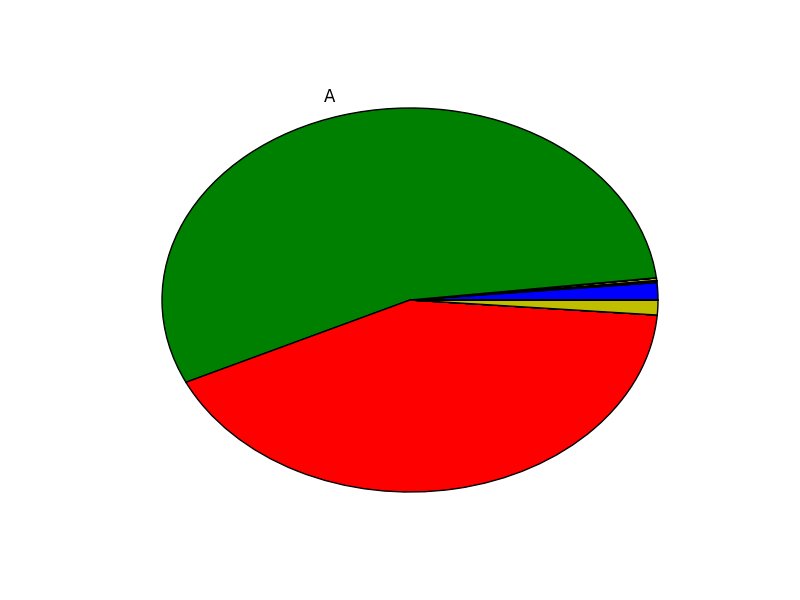
\includegraphics[width=0.5\textwidth]{%
      ../output/marto-casa-3hs-s1-pie.png}
      \vspace{-2em}
      \caption{S$_1$: Casa - Torta}
      \label{marto-casa-3hs-s1-pie}
    \end{center}\end{figure}

    %------------------------------------------------------------------
    % HISTOGRAMA CASA
    %------------------------------------------------------------------
    \begin{figure}[ht]\begin{center}
      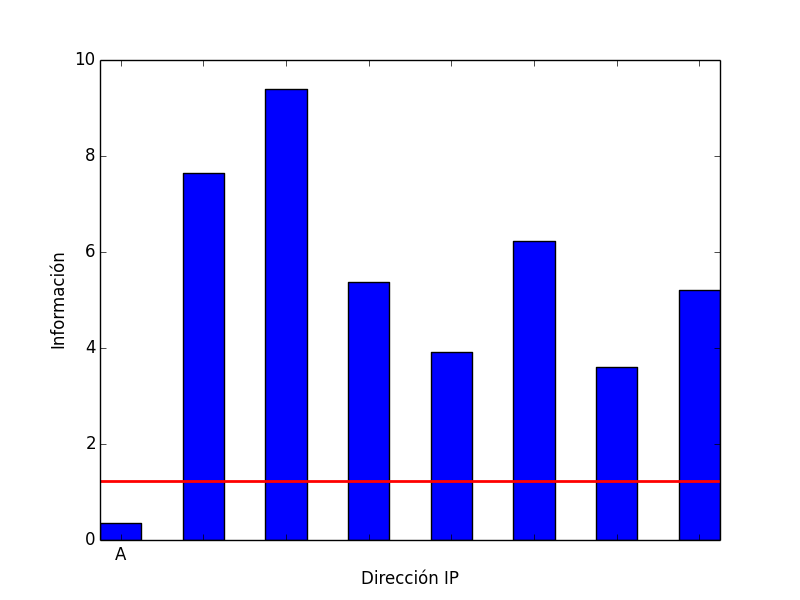
\includegraphics[width=0.5\textwidth]{%
      ../output/marto-casa-3hs-s1-histogram.png}
      \vspace{-2em}
      \caption{S$_1$: Casa - Histograma}
      \label{marto-casa-3hs-s1-histogram}
    \end{center}\end{figure}

    %------------------------------------------------------------------
    % GRAFO CASA
    %------------------------------------------------------------------
    \begin{figure}[ht]\begin{center}
      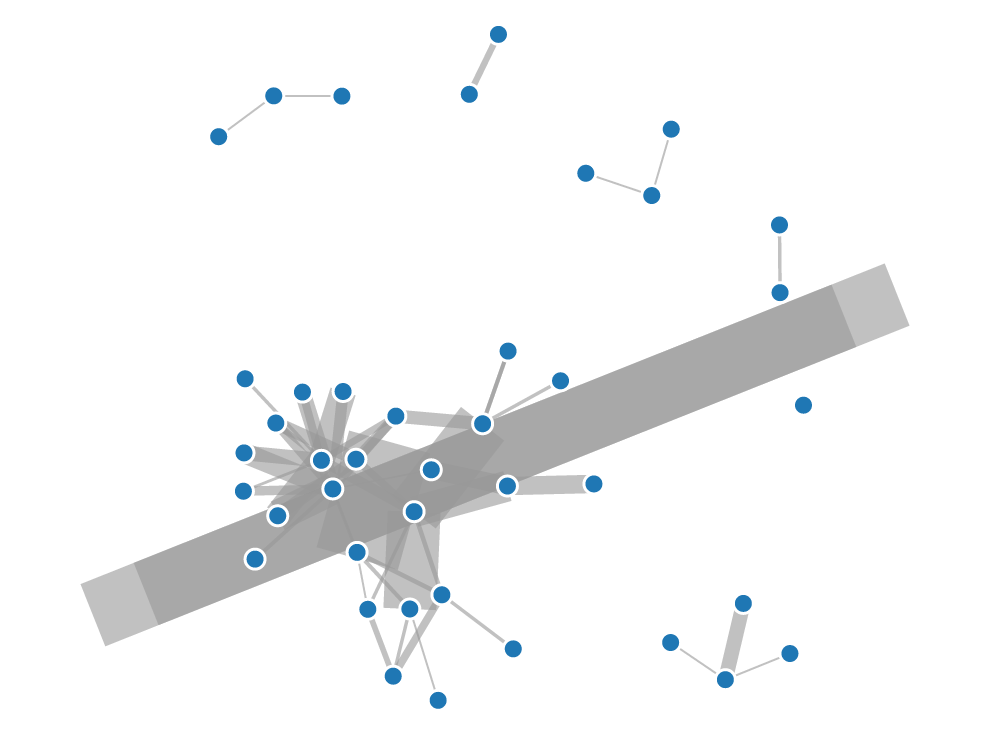
\includegraphics[width=0.5\textwidth]{%
      ../output/marto-casa-3hs-graph.png}
      \vspace{-2em}
      \caption{S$_1$: Casa - Grafo}
      \label{marto-casa-3hs-graph}
    \end{center}\end{figure}

  La ip que más aparece en los paquetes de tipo \texttt{ARP}, dentro
  del campo \textit{destino}, es la 190.168.1.100, tal como se observa
  en la figura \ref{marto-casa-3hs-s1-pie}. Esta ip al ser la que más
  aparece dentro de las comunicaciones, será un nodo distinguido, por
  lo que será la que menos información aporte. Esto se ve reflejado en
  la figura \ref{marto-casa-3hs-s1-histogram}, en donde la información
  que brinda la ip 190.168.1.100 (representada como A) queda por
  debajo de la entropía de la fuente, la cual es 1.24.

  Las direcciones ip que no son distinguidas tienen frecuencias y
  probabilidades de aparición muy similares, aportando así cantidades
  similares de información. Esto se puede observar en la figura
  \ref{marto-casa-3hs-s1-histogram}.

  En la figura \ref{marto-casa-3hs-graph} se observan 7 componentes
  conexas (hay 7 subconjuntos de ip's que intercambian información
  sólo entre sí y no con las demas ip's de la red). También se puede
  observar que hay dos pares de dos nodos (direcciones ip) que están
  unidos por una arista de un grosor enorme. Se deduce que estos pares
  de  nodos intercambian entre sí una cantidad muy grande de paquetes.
  El grafo muestra nodos de la red que recibieron o emitieron
  paquetes, mientras que en el histograma sólo mostramos a los nodos
  que \texttt{recibieron} paquetes ya que los símbolos que
  consideramos son el campo \texttt{destino} de los paquetes. Es por
  esto que en el grafo aparecen representados más nodos de la red que
  en el histograma.

  %------------------------------------------------------------ --------
  % SUBSECTION III-B: TECHINT
  %--------------------------------------------------------------------
  \subsection{Techint}

  Las condiciones en las que se midió fueron las mismas a la detallada
  en la introducción, solamente se cambió la fuente utilizada y se
  filtraron los paquetes segun el tipo \texttt{ARP}.

    %------------------------------------------------------------------
    % TORTA TECHINT
    %------------------------------------------------------------------
    \begin{figure}[ht]\begin{center}
      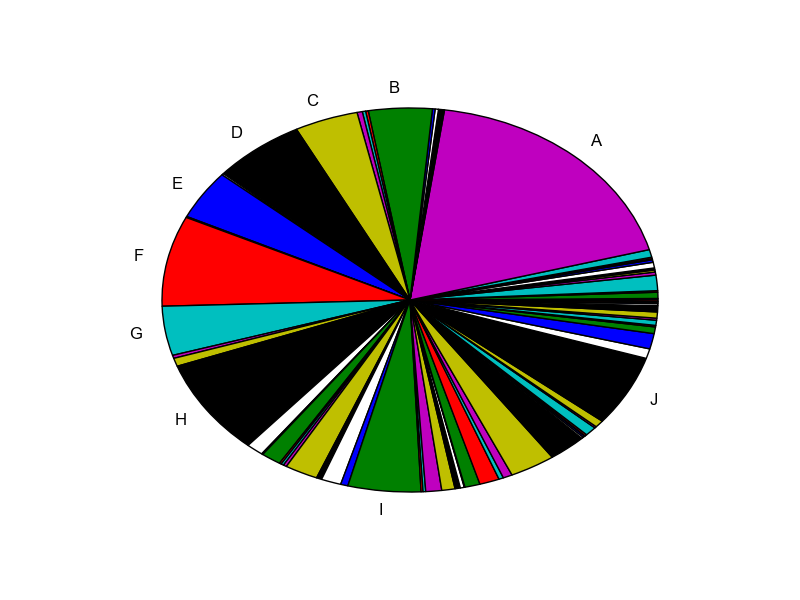
\includegraphics[width=0.5\textwidth]{%
      ../output/techint-s1-pie.png}
      \vspace{-2em}
      \caption{S$_1$: Techint - Torta}
      \label{techint-s1-pie}
    \end{center}\end{figure}

    %------------------------------------------------------------------
    % HISTOGRAMA TECHINT
    %------------------------------------------------------------------
    \begin{figure}[H]\begin{center}
      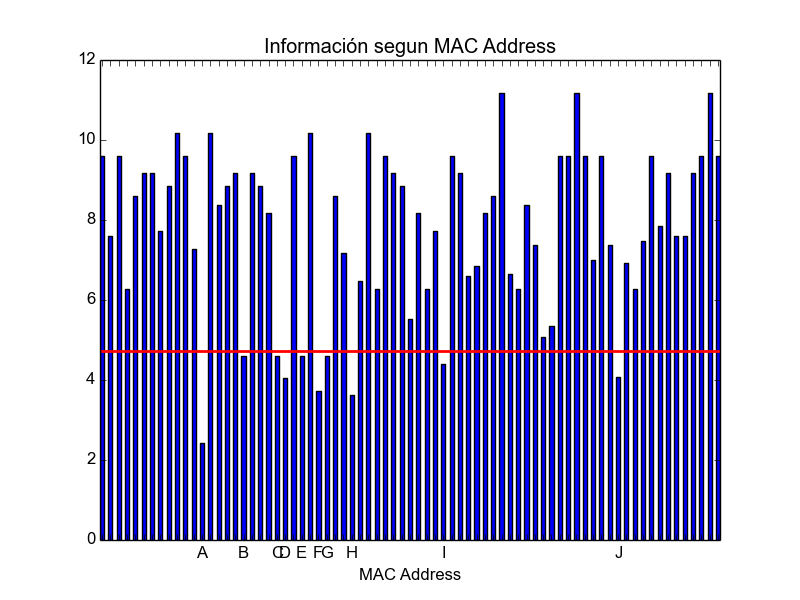
\includegraphics[width=0.5\textwidth]{%
      ../output/techint-s1-histogram.png}
      \vspace{-2em}
      \caption{S$_1$: Techint - Histograma}
      \label{techint-s1-histogram}
    \end{center}\end{figure}

    %------------------------------------------------------------------
    % GRAFO TECHINT
    %------------------------------------------------------------------
    \begin{figure}[H]\begin{center}
      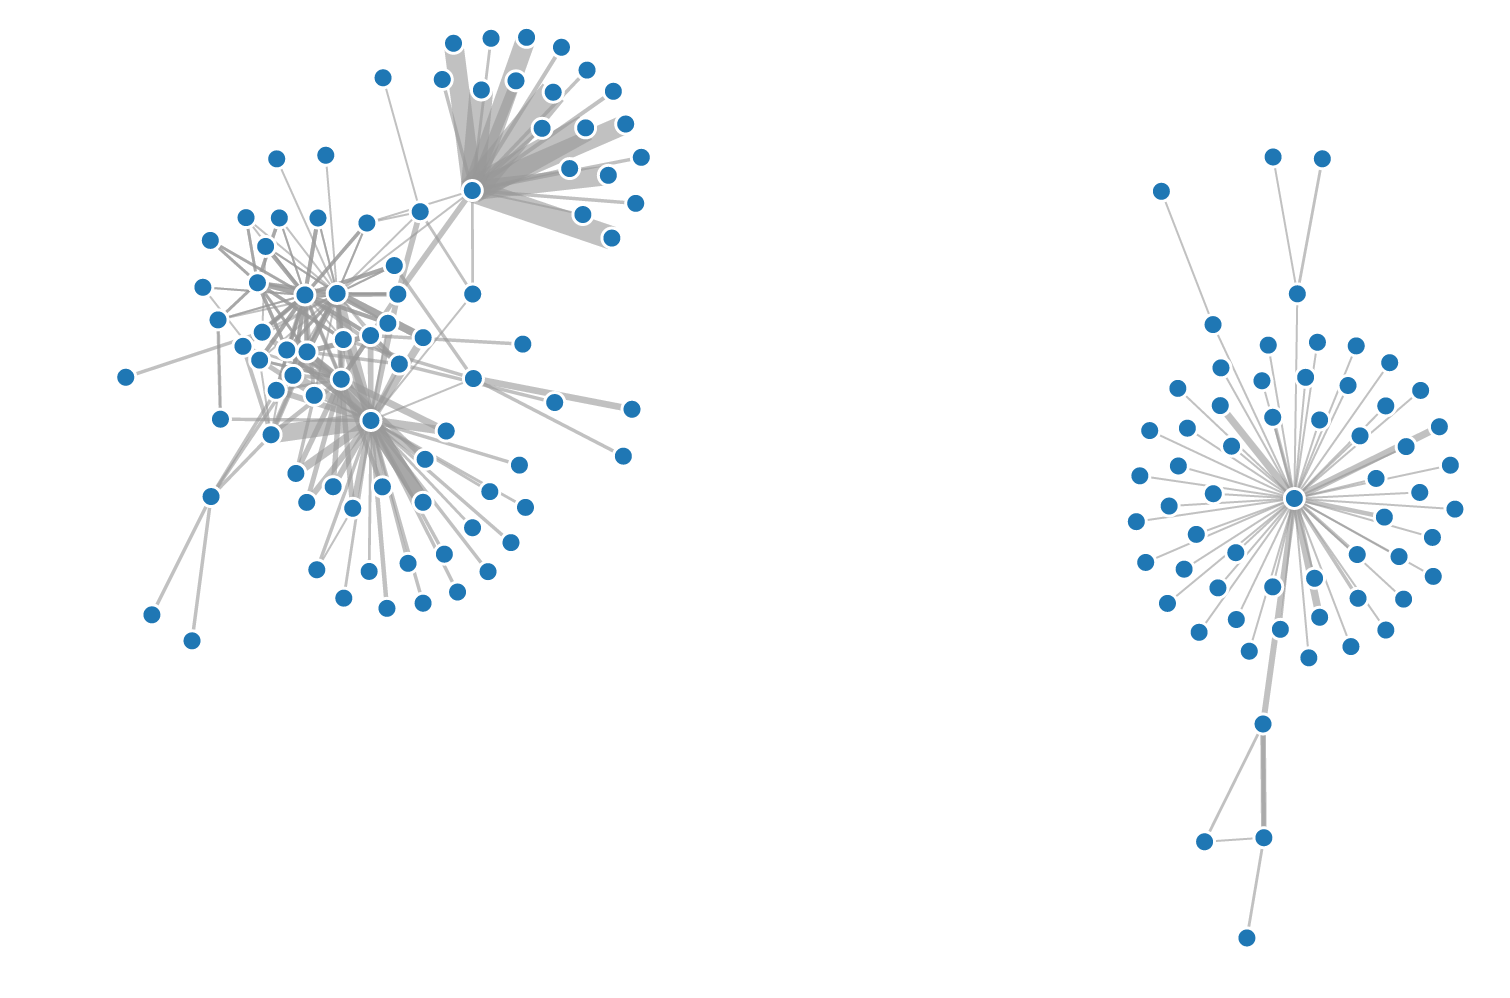
\includegraphics[width=0.5\textwidth]{%
      ../output/techint-s1-graph.png}
      \vspace{-2em}
      \caption{S$_1$: Techint - Grafo}
      \label{techint-s1-graph}
    \end{center}\end{figure}


  En este caso se encontró un subconjunto de nodos distinguidos, los
  cuales presentan una frecuencia significativamente mayor en
  comparación con el resto de los nodos. Esto se puede observar en la
  figura \ref{techint-s1-pie}.

  Todos estos nodos aportaron un información menor a la entropía de la
  fuente, la cual fue de 4.73. Estos estan enumerados con letras de la
  A a la J, formando así un subconjunto con 10 nodos distinguidos, tal
  como se ve en la figura \ref{techint-s1-histogram}. Dentro de estos
  nodos, se observa uno en particular nombrado como A (cuya ip es
  172.23.135.254), que aparece con una frecuencia mayor al resto
  (18\%), lo que como consecuencia aportará menor cantidad de
  información.

  También realizamos un grafo a partir de los datos de forma similar a
  la hecha en la red \emph{Casa}. En este caso se pueden observar dos
  componentes conexas. En ambas componentes se observa que hay uno o
  más \texttt{nodos especiales}, que están conectados con una cantidad
  grande de nodos que sólo se conectan con este. Estos nodos son nodos
  correspondientes a los símbolos destacados (que se encuentran por
  debajo de la entropía) en el histograma de la figura
  \ref{techint-s1-histogram}. Luego, consideramos que es esperable que
  estos símbolos (o al menos alguno/s) de estos se correspondan con la
  dirección ip de routers presentes en la red.

  %--------------------------------------------------------------------
  % SUBSECTION III-C: HYUNDAI
  %--------------------------------------------------------------------
  \subsection{Hyundai}

Se observan dos nodos distinguidos, nombrados como A y B, cuyas
frecuencias de aparición son las mayores. A su vez se puede distinguir una
jerarquía en la que además de estos nodos primarios existe una serie de
nodos de segundo nivel en cuanto a su frecuencia, tal como se observa en
la figura \ref{hyundai-s1-histogram}.

Esta jerarquía también es observable en la figura \ref{hyundai-graph}, en
donde hay un nodo central bien marcado, y otros nodos importantes  en su periferia más
cercana.

Segun sabemos del entorno en donde fue realizada la medición, esto es
posiblemente una consecuencia de la topología de la red en donde se
realizó la medición, en particular pudimos corroborar que muchas de las
ips correspondientes a los nodos pertenecen a servidores, que brindan
servicios activos a todo el resto de las máquinas de la empresa. De esta
forma es comprensible que los mismos tengan una gran cantidad de
solicitudes \texttt{ARP}.


    %------------------------------------------------------------------
    % TORTA HYUNDAI
    %------------------------------------------------------------------
    \begin{figure}[ht]\begin{center}
      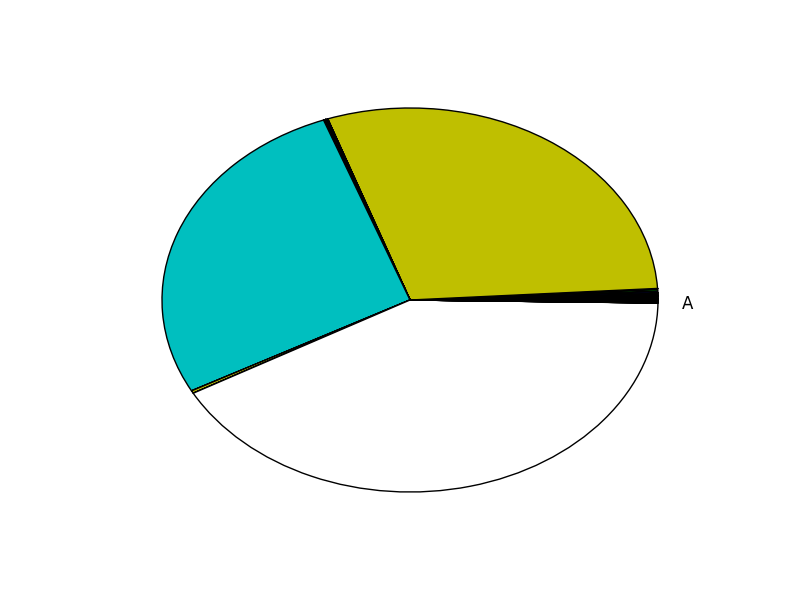
\includegraphics[width=0.5\textwidth]{%
      ../output/hyundai-s1-pie.png}
      \vspace{-2em}
      \caption{S$_1$: Hyundai - Torta}
      \label{hyundai-s1-pie}
    \end{center}\end{figure}

    %------------------------------------------------------------------
    % HISTOGRAMA HYUNDAI
    %------------------------------------------------------------------
    \begin{figure}[H]\begin{center}
      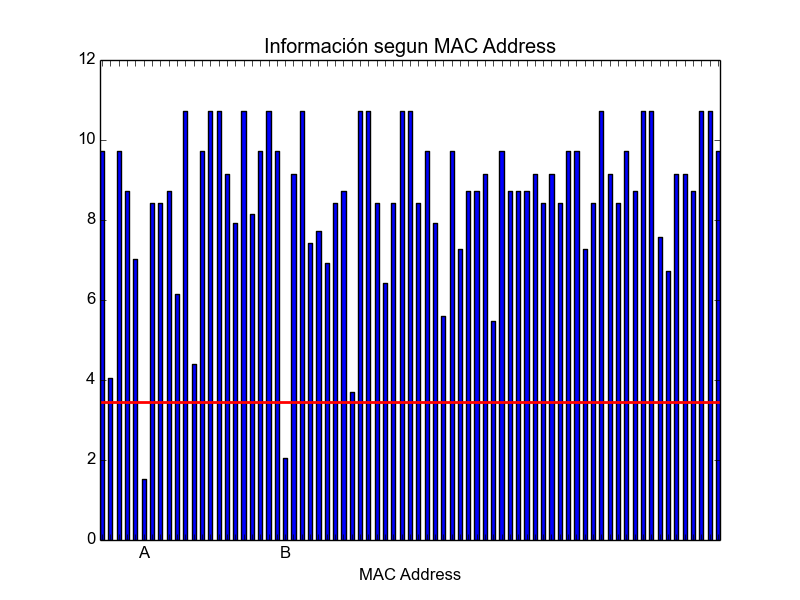
\includegraphics[width=0.5\textwidth]{%
      ../output/hyundai-s1-histogram.png}
      \vspace{-2em}
      \caption{S$_1$: Hyundai - Histograma}
      \label{hyundai-s1-histogram}
    \end{center}\end{figure}

    %------------------------------------------------------------------
    % TOPOLOGÍA DE RED HYUNDAI
    %------------------------------------------------------------------
    \begin{figure}[ht]\begin{center}
      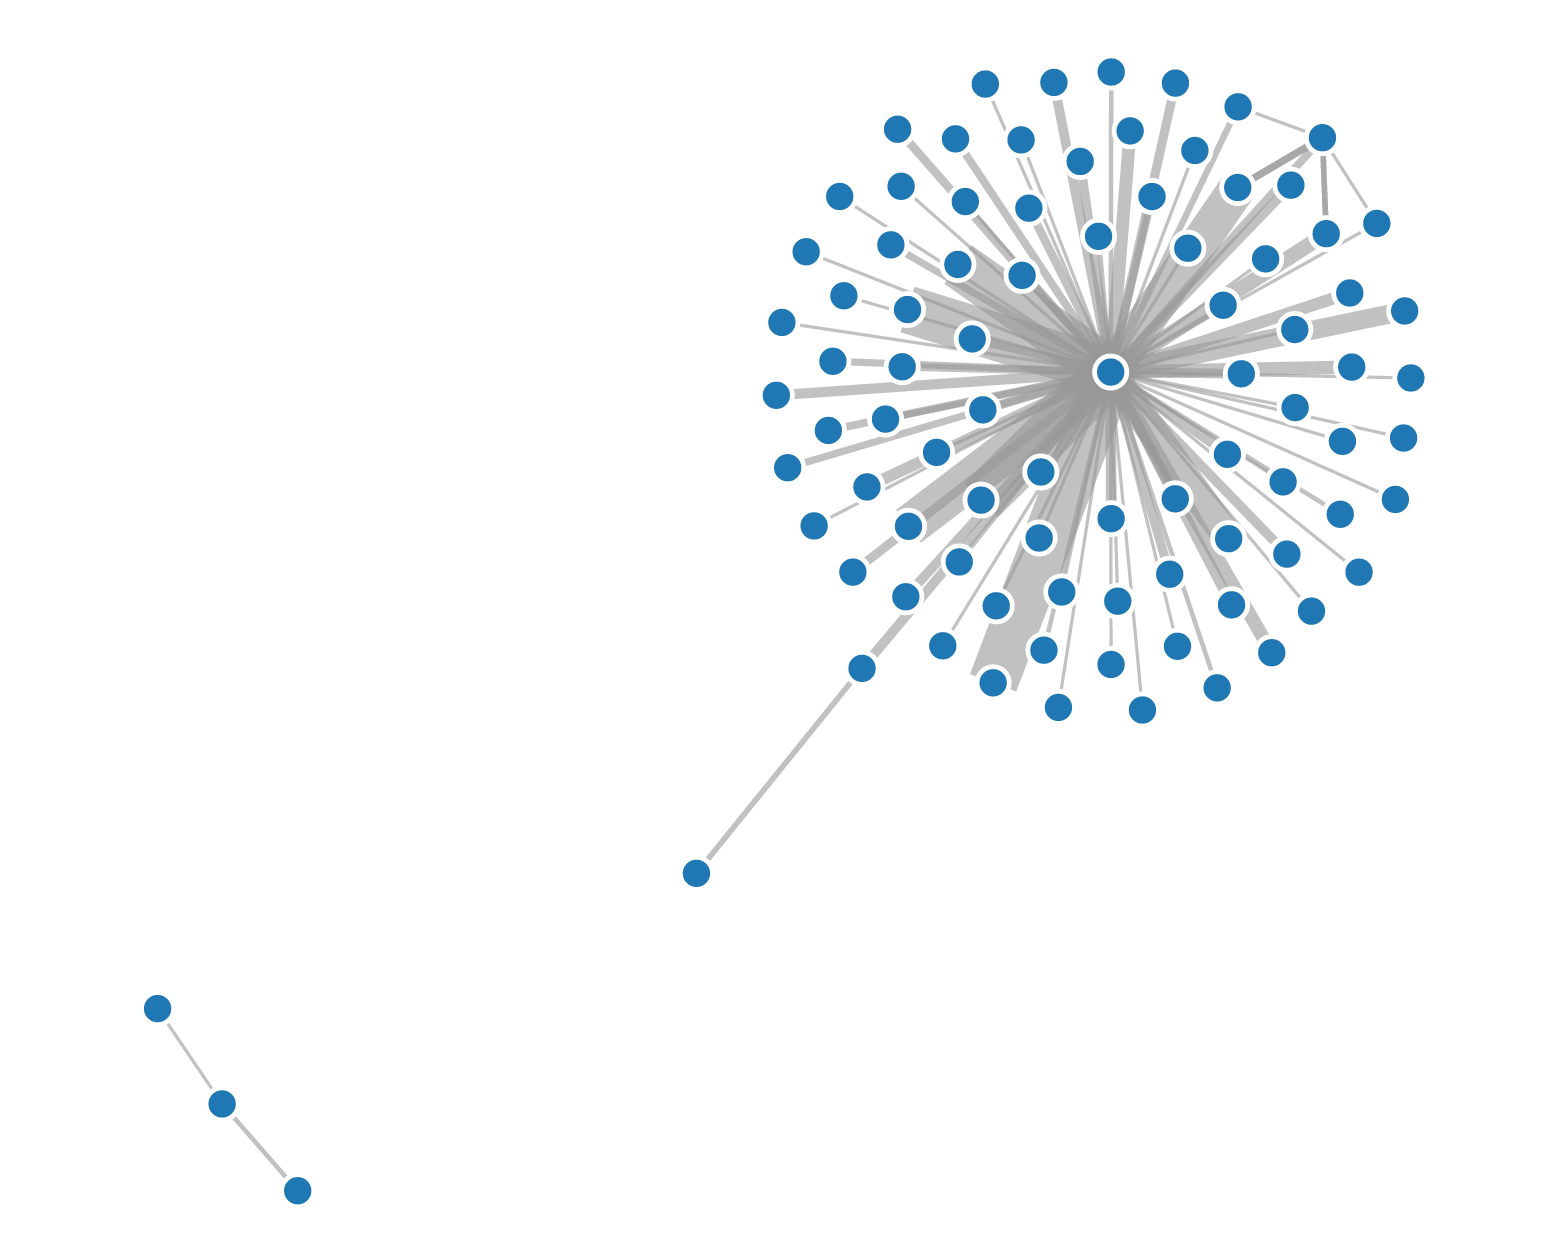
\includegraphics[width=0.5\textwidth]{%
      ../output/hyundai-graph.png}
      \vspace{-2em}
      \caption{S$_1$: Hyundai - Topología de la Red}
      \label{hyundai-graph}
    \end{center}\end{figure}

  %--------------------------------------------------------------------
  % SUBSECTION III-D: LABORATORIOS DC
  %--------------------------------------------------------------------
  \subsection{Laboratorios DC}

  Las condiciones en las que se midió fueron las mismas a la detallada
  en la introducción, solamente se cambió la fuente utilizada y se
  filtraron los paquetes segun el tipo \texttt{ARP}.

    %------------------------------------------------------------------
    % TORTA LABOS-DC
    %------------------------------------------------------------------
    \begin{figure}[ht]\begin{center}
      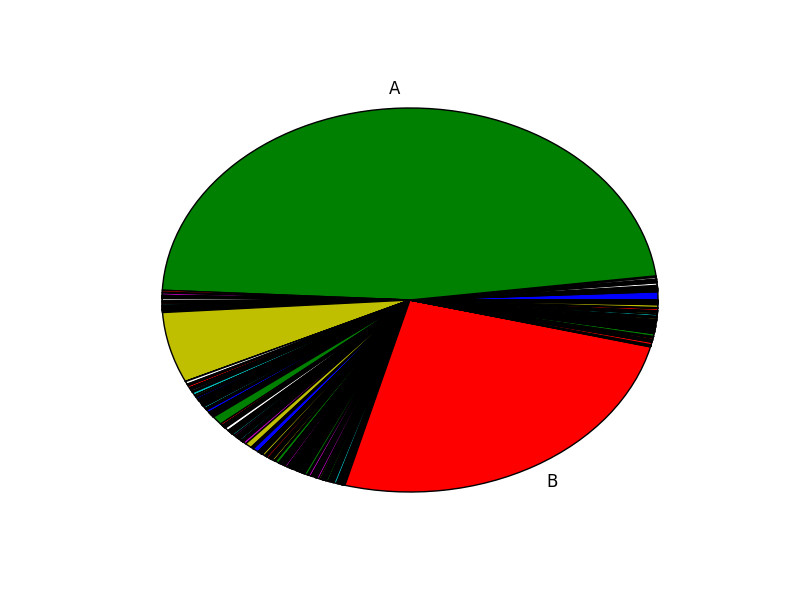
\includegraphics[width=0.5\textwidth]{%
      ../output/labos-dc-30m-s1-pie.png}
      \vspace{-2em}
      \caption{S$_1$: Laboratorios DC - Torta}
      \label{labos-dc-30m-s1-pie}
    \end{center}\end{figure}

    %------------------------------------------------------------------
    % HISTOGRAMA LABOS-DC
    %------------------------------------------------------------------
    \begin{figure}[ht]\begin{center}
      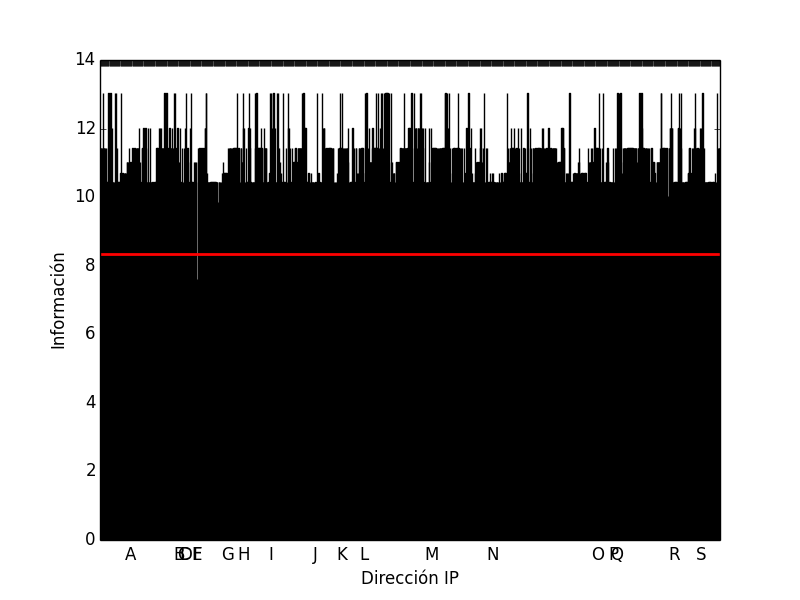
\includegraphics[width=0.5\textwidth]{%
      ../output/labos-dc-30m-s1-histogram.png}
      %\vspace{-2em}
      \caption{S$_1$: Laboratorios DC - Histograma}
      \label{labos-dc-30m-s1-histogram}
    \end{center}\end{figure}

    %------------------------------------------------------------------
    % GRAFO LABOS-DC
    %------------------------------------------------------------------
    \begin{figure}[ht]\begin{center}
      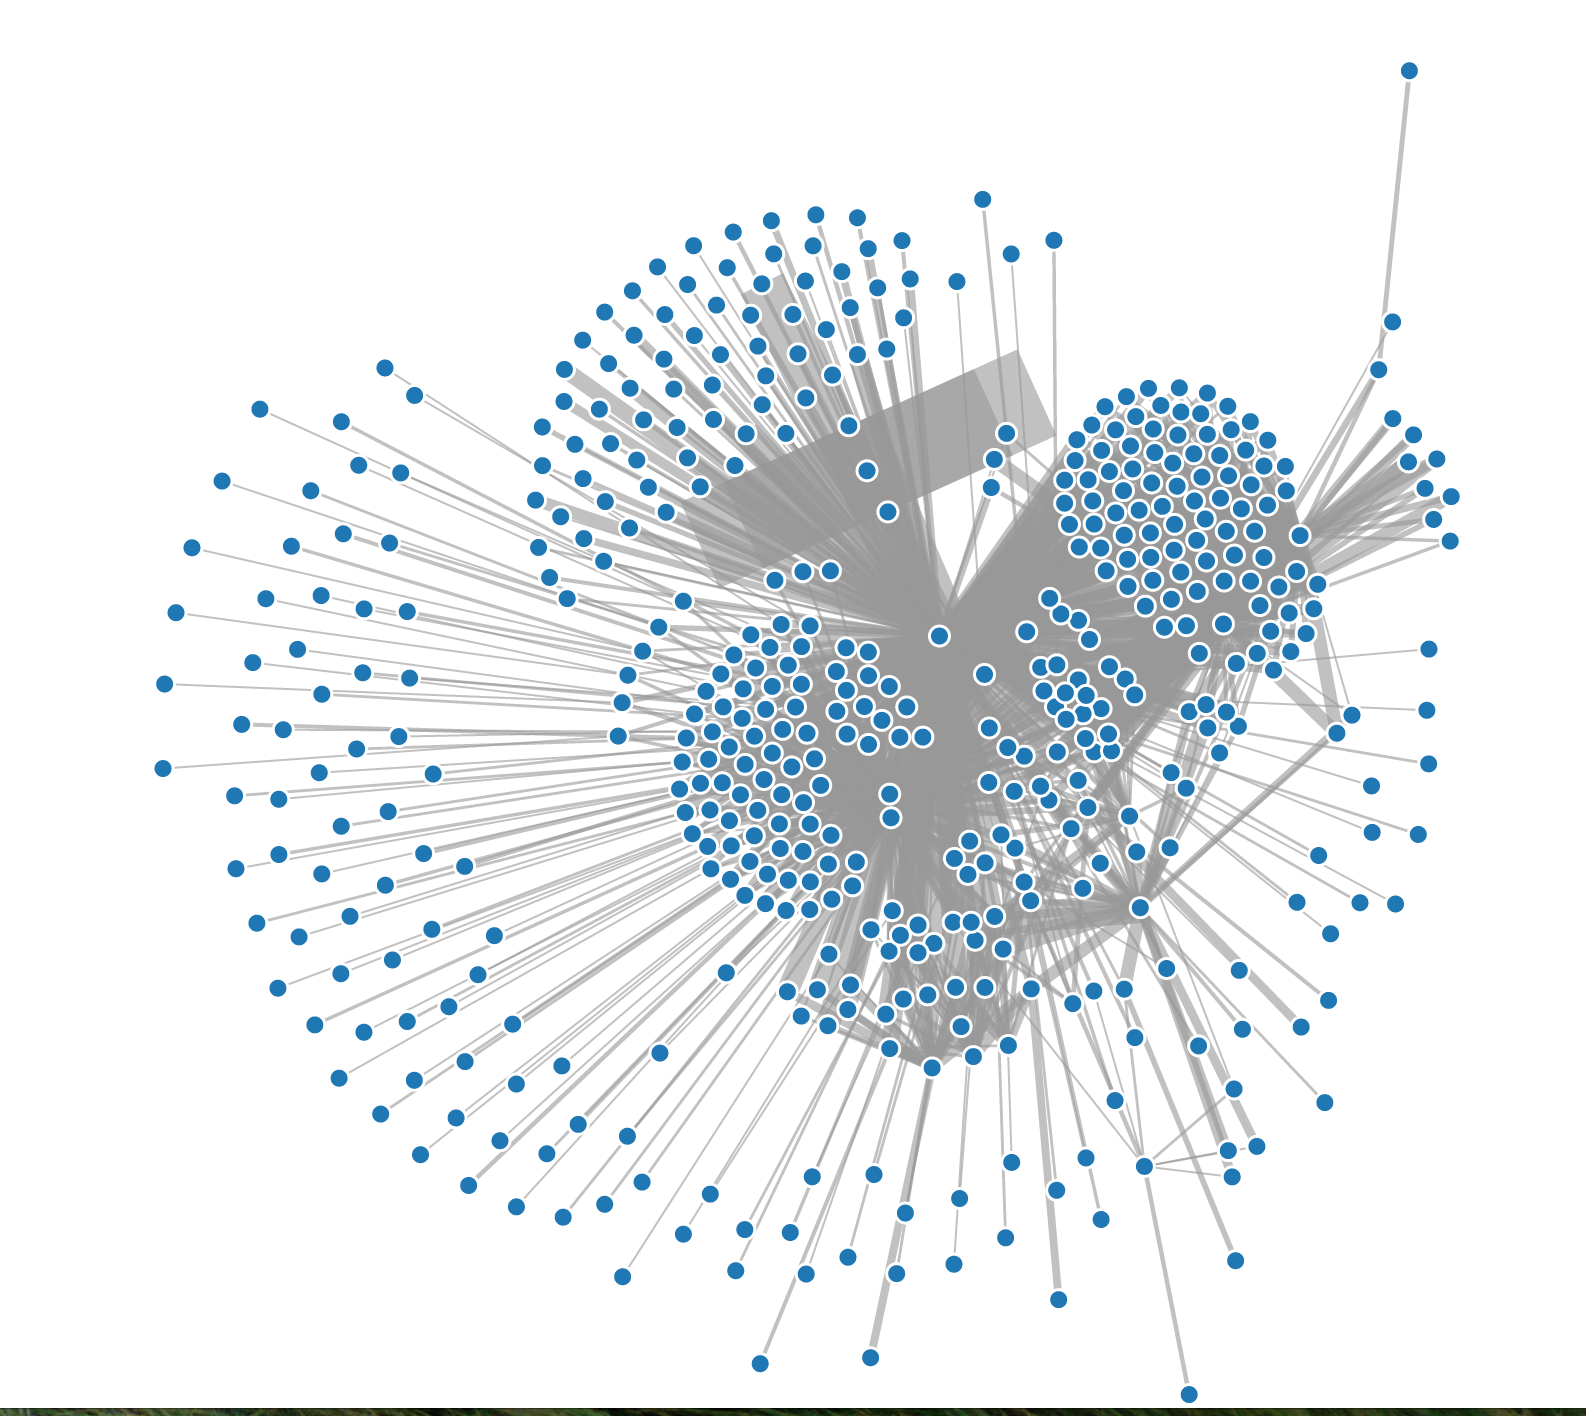
\includegraphics[width=0.5\textwidth]{%
      ../output/labos-dc-30m-graph.png}
      %\vspace{-2em}
      \caption{S$_1$: Laboratorios DC - Grafo}
      \label{labos-dc-30m-graph}
    \end{center}\end{figure}

  En esta medición se encontraron 20 nodos distinguidos. Dentro de
  este subconjunto se observó un nodo en particular, el S, como se
  puede observar en la figura \ref{labos-dc-30m-s1-pie}. Sin embargo,
  en la figura \ref{labos-dc-30m-s1-histogram} no se puede apreciar
  que aporta poca información y queda debajo de la entropía (8.33),
  puesto que la cantidad de símbolos graficados es muy grande,
  haciendo que el ancho de la columna que lo representa en el
  histograma no sea visible. Sí son visibles el conjunto de nodos
  B,C,D,E y F, que están todos por debajo de la entropía y casualmente
  cada uno aporta casi la misma cantidad de información.

  También se observó en el histograma de la figura
  \ref{labos-dc-30m-s1-histogram} que a simple vista hay
  aproximadamente 4 niveles de cantidad de información provista por
  los símbolos, y que hay poca variación en la cantidad de información
  provista por prácticamente todos ellos (excepto por el símbolo S,
  que aporta 2.44 de información).

  Finalmente, realizamos un grafo de igual forma que en las mediciones
  anteriores. En este caso se observa una única componente conexa, con
  muchos nodos frontera conectados mediante una arista con pocos nodos
  centrales. Los gráficos sigieren que estos se correspondan con los
  símbolos que están por debajo de la entropía en el histograma de la
  figura \ref{labos-dc-30m-s1-histogram}. Al igual que en las
  mediciones ya analizadas, será esperable que estos símbolos sean la
  dirección ip de dispositivos (nodos) destacados en la red local
  estudiada (por ejemplo, podrían ser routers).


  %--------------------------------------------------------------------
  % SUBSECTION III-F: Conclusión
  %--------------------------------------------------------------------
  \subsection{Conclusión de las mediciones}

  En todas las mediciones se encontraron indicios que parecen responder a una topología lógica con forma de estrella subyacente. Esto se condice con lo visto en clase ya que responde a las metodologías de ruteo explicadas. Por ejemplo, routers en cascada o subredes bien definidas.

  A diferencia de la fuente anterior, se encontraron en todos los casos más de un símbolo distinguido. Aparentemente, la distribución de probabilidades de esta fuente tiene una estructura jerárquica.

\newpage
%----------------------------------------------------------------------
% SECTION IV: Conclusión
%----------------------------------------------------------------------
\section{Conclusión}

Para finalizar, podemos decir que nos divirtió mucho
la realización de este TP, ya que fuimos capaces de
internalizarnos en el funcionamiento de las redes de
área local (LAN) que usamos desde temprana edad
prácticamente todos los días de nuestras vidas.

Pudimos entender que para la comunicación entre un
servidor y un host, se tienen que efectuar una serie
de intercambios de datos entre distintas capas de datos
de la red. También, utilizamos lo aprendido en clase
de teoría de la información para analizar características
de las redes analizadas.

Como ya fue dicho, sobre un mismo conjunto de mediciones
de red, definimos dos fuentes distintas: $S$ y $S_1$.
Pudimos observar que las entropías presentadas en los
experimentos sobre la fuente $S$ fueron menores que las
presentadas sobre la fuente $S_1$. A partir de esto, y
aplicando lo que nos enseñó Shannon de teoría de la
información, podemos concluir que la fuente $S$ es
\emph{más compresible} que la fuente $S_1$. Es decir, que
en teoría se podría lograr una codificación óptima de longitud
media menor de la fuente $S$.

Además, en todos los experimentos (sobre ambas fuentes),
identificamos nodos distinguidos (por debajo de la entropía de
la fuente).

El trabajo práctico tuvo un componente no presente en trabajos previos que fue la toma de mediciones en el entorno. Esto nos permitió realizar inferencias sobre el mundo real.



\end{document}
